\documentclass[]{scrreprt}
\usepackage{amsmath,amsfonts,graphicx}
\usepackage{multirow}
\usepackage{pslatex}
\usepackage{tabularx}
\usepackage{comment}
\usepackage{xspace}
\usepackage{array}

\usepackage{hyperref}

\usepackage{caption}
\DeclareCaptionFont{white}{\color{white}}
\DeclareCaptionFormat{listing}{\colorbox{gray}{\parbox{\textwidth}{#1#2#3}}}

\graphicspath{
{figures/}
}

\newcommand{\uo}{\mbox{UO\textsubscript{2}}\xspace}

\setcounter{secnumdepth}{3}

\newcommand{\si}{\sigma}
\newcommand{\mand}{\ \ \ \mbox{and}\ \ \ }
\newcommand{\pl}{\partial}
\newcommand{\ha}{\mbox{$\frac{1}{2}$}}
\newcommand{\thetac}{\theta^{\mathrm{c}}}
\newcommand{\thetarel}{\theta^{\mathrm{rel}}}
\newcommand{\ep}{\epsilon}
\newcommand{\ga}{\gamma}
\newcommand{\spa}{\ \ \ }
\newcommand{\non}{\nonumber}
\newcommand{\de}{\delta}
\newcommand{\ka}{\kappa}
\newcommand{\la}{\lambda}
\newcommand{\tr}{\mbox{Tr}\,}
\newcommand{\al}{\alpha}
\newcommand{\be}{\beta}
\newcommand{\cd}{\cdot}

\begin{document}


\title{Cosserat Test suite}
\author{CSIRO}
\maketitle

\abstract{Tests involving Cosserat mechanics are described.  The
  notation is defined in the Theory manual.}

\tableofcontents

\chapter{Cosserat glide: elasticity}

Forest\footnote{S Forest "Mechanics of Cosserat media An
  introduction".  Available from
  http://citeseerx.ist.psu.edu/viewdoc/download?doi=10.1.1.154.4476\&rep=rep1\&type=pdf}
describes a ``glide'' test of Cosserat elasticity in his Appendix A.
The test involves a 3D material, but all quantities are assumed to be
functions of the $x_{2} = y$ direction only.
The displacement field, $u$, and Cosserat rotation, $\thetac$
are assumed to obey
\begin{eqnarray}
u_{i} & = & (u_{x}(y),\ 0,\ 0) \ , \\
\thetac_{i} & = & (0,\ 0,\ \thetac_{z}(y)) \ .
\end{eqnarray}
These mean that the strain tensor, $\gamma$, and curvature tensor, $\kappa$, are
\begin{eqnarray}
\gamma = \left(
\begin{array}{ccc}
0 & \thetac_{z} + \nabla_{y}u_{x} & 0 \\
-\thetac_{z} & 0 & 0 \\
0 & 0 & 0
\end{array}
\right)
&&
\kappa = \left(
\begin{array}{ccc}
0 & 0 & 0 \\
0 & 0 & 0 \\
0 & \nabla_{y}\thetac_{z} & 0
\end{array}
\right)
\end{eqnarray}
The solution below has boundary conditions $u_{x}(0) = 0 =
\thetac_{z}(y)$.

The stress and couple-stress tensors are assumed to be zero, except for
the following components:
\begin{eqnarray}
\sigma_{yx} & \neq & 0 \ , \\
m_{zy} & \neq & 0 \ .
\end{eqnarray}
This is depicted in Figure~\ref{glide.fig}.
If standard (non-Cosserat, Cauchy) elasticity were being
used, the solution is the trivial $u_{x} = 0$.  However, using
Cosserat elasticity a nontrivial solution is found.
Physically this setup corresponds to a 3D object subjected to a moment $m_{zy}$ that
rotates the Cosserat grains.

\begin{figure}[htb]
\begin{center}
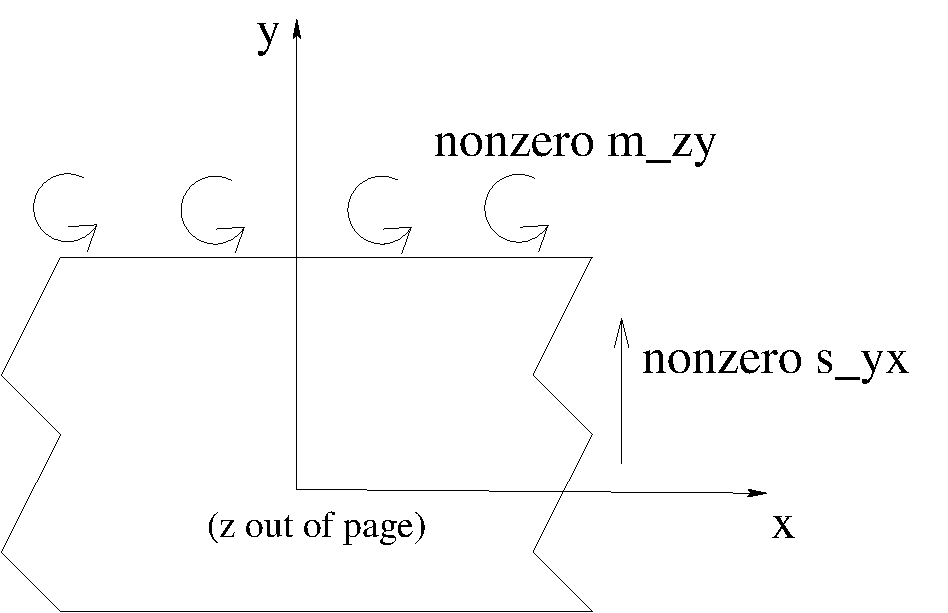
\includegraphics[width=6cm]{glide_fig.pdf}
\caption{The Cosserat glide experiment}
\label{glide.fig}
\end{center}
\end{figure}

Isotropic elasticity is assumed, with the additional assumption that
the couple-stress equation only involves two moduli:
\begin{eqnarray}
\si_{ij} & = & \la\de_{ij}\tr\ga + 2\mu\ga_{(ij)} + 2\al\ga_{[ij]} \ ,
\non \\
m_{ij} & = & \be\de_{ij}\tr\ka + 2\ep\ka_{(ij)} + 2\ep\ka_{[ij]} \ .
\end{eqnarray}
With these assumptions, the moment and force balance equations reduce
to a second-order ODE that has solution
\begin{eqnarray}
\thetac_{z} & = & B\sinh(\omega_{e}y) \ , \\
u_{x} & = & \frac{2 \al B}{\omega_{e}(\mu + \al)}(1 -
\cosh(\omega_{e}y)) \ , \\
m_{zy} & = & 2B\epsilon \omega_{e}\cosh(\omega_{e}y) \ , \\
\sigma_{yx} & = & -\frac{4\mu\al}{\mu + \al}B\sinh(\omega_{e}y)
\end{eqnarray}
with $B$ being an arbitrary constant of integration, and
\begin{equation}
\omega_{e} = \sqrt{\frac{2\mu\al}{\epsilon(\mu + \al)}} \ .
\end{equation}
Forest's notation is slightly different: for $\al$ he writes $\mu_{c}$,
and for $\epsilon$ he writes $\beta$.

The MOOSE simulation uses 100 elements in the $y$ direction, with
$\mu=2$, $\al=3$ and $\epsilon=0.6$.  This gives $w_{e}=2$.  Preset
boundary conditions at $y=0$ and $y=1$ are used, and the system
relaxes to the equilirium solution within 1 iteration.
Figure~\ref{glide_elast.fig} reveals that the MOOSE simulation agrees
with expectations.  The displacements agree well for the 100-element
simulation, but the stress components agree less well (this is not
really observable to the eye in Figure~\ref{glide_elast.fig}) and even a
non-zero $\sigma_{xy}$ appears.  However, as the number of elements
is increased, the stresses tend to the analytical formulae given above.

\begin{figure}[htb]
\begin{center}
\begin{tabular}{cc}
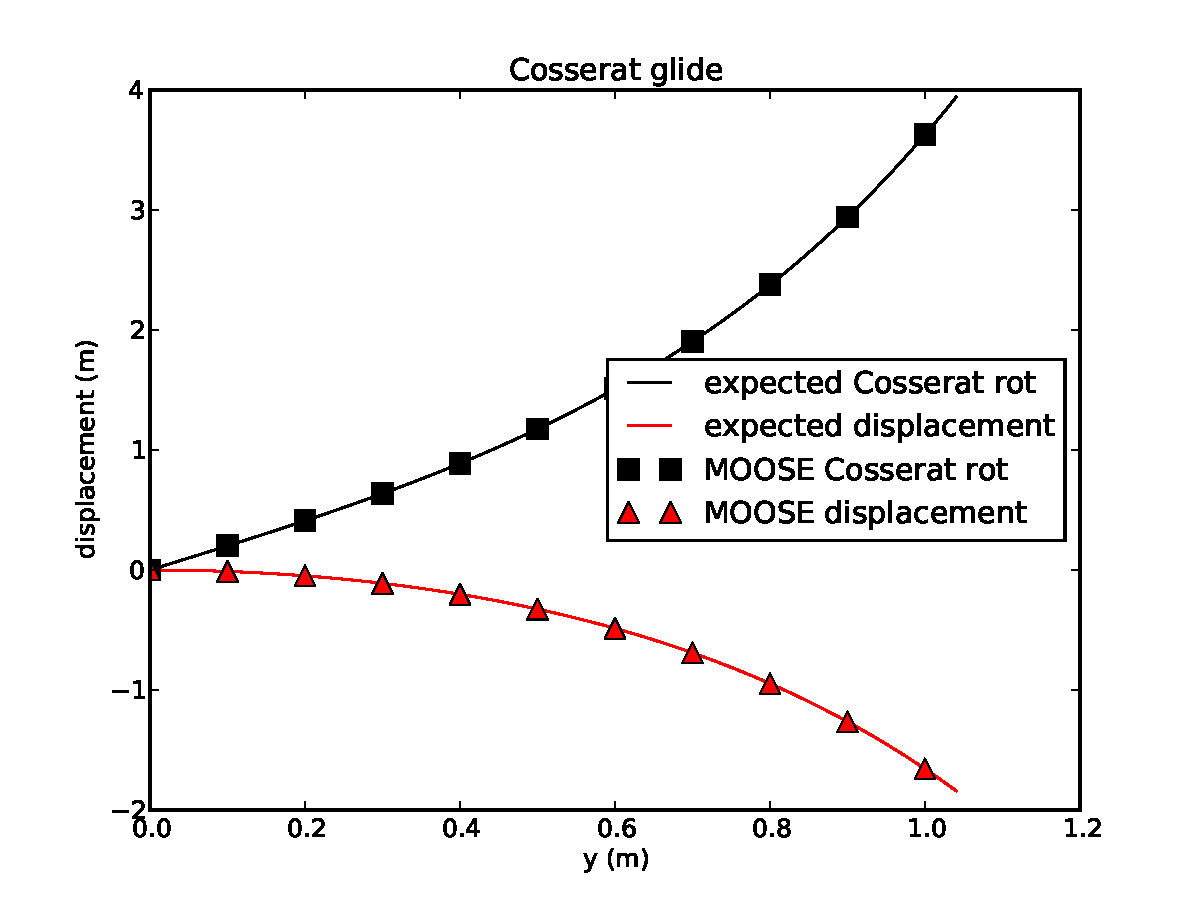
\includegraphics[width=8cm]{cosserat_glide_disp.pdf}
&
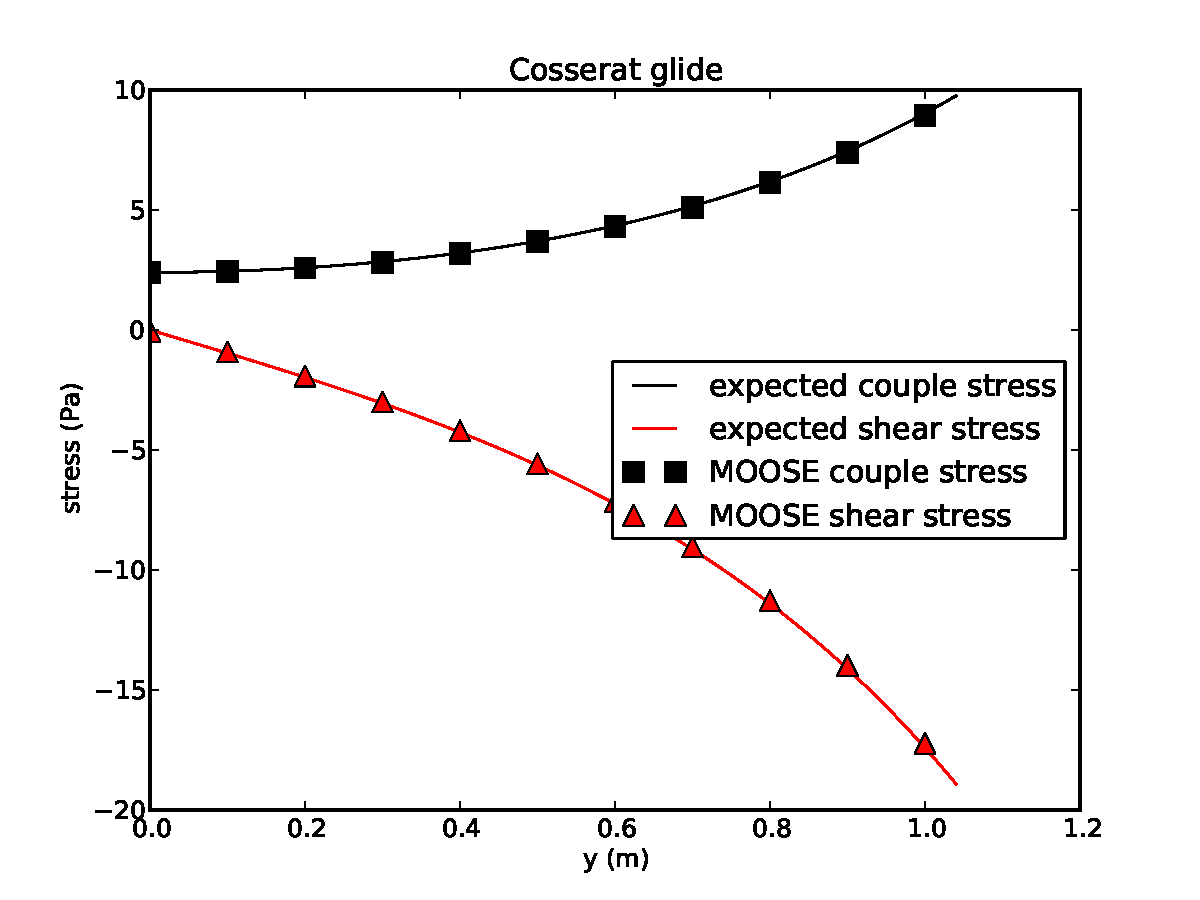
\includegraphics[width=8cm]{cosserat_glide_stress.pdf}
\end{tabular}
\caption{Results from the elastic Cosserat glide test.  Left:
  displacements.  Right: stresses}
\label{glide_elast.fig}
\end{center}
\end{figure}


\chapter{Cosserat tension}

This is a simple test where a 3D sample is subjected to a normal load
on its top surface.  The sample is allowed to shrink in directions
perpendicular to the force, via the Poisson's ratio.  Specifically,
all components of the stress tensor are zero except for
\begin{equation}
\sigma_{22} \neq 0 \ ,
\end{equation}
(which is constant).
There are no Cosserat rotations involved:
\begin{equation}
m = 0 = \kappa \ .
\end{equation}
A general isotropic elasticity tensor is assumed so that the
constitutive relation reads
\begin{equation}
\si_{ij} = \la\de_{ij}\tr\ga + 2\mu\ga_{(ij)} + 2\al\ga_{[ij]} \ .
\end{equation}
The solution is identical to the standard (non-Cosserat) case, which
is independent of $\al$, and has strain components
\begin{equation}
\epsilon_{22} = \frac{(\la + \mu)}{\mu(3\la + 2\mu)}\sigma_{22}
\ \ \ \mbox{and}\ \ \
\epsilon_{11} = \epsilon_{33} = -\frac{\la}{2(\mu + \la)}\epsilon_{22}
\ .
\end{equation}
MOOSE generates this solution exactly.


\chapter{Beam bending 1}

A cantilever beam is held fixed at one end, and bent by a surface
traction applied at its other end.  As shown in
Figure~\ref{beam_cant.fig}, the beam has length $L$, width $2c$, and a
surface traction of $\tau$ is applied to its free end.  In this
section, the beam will be modelled using a layered Cosserat material,
but with the Cosserat-joint normal and shear stiffnesses being very
large.  This means that that Cosserat theory should be identical to
standard (non-Cosserat) elasticity.

\begin{figure}[htb]
\begin{center}
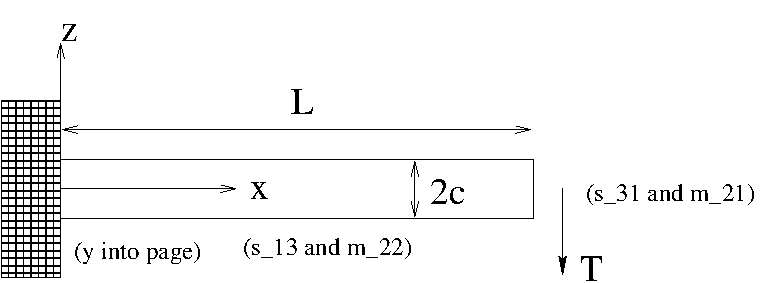
\includegraphics[width=11cm]{beam_cantilever.pdf}
\caption{A cantilever beam of length $L$ and width $2c$ is held fixed
  at one end ($x=0$) and subjected to a surface traction $\tau$ at the
  other end ($x=L$).  For reference in the text, some stress and
  moment-stress components have been shown: $\sigma_{31}$ acts on the
  $x=L$ plane in the $z$ direction; $m_{21}$ acts on the $x=L$ plane to
  rotate around the $y$ axis; $\sigma_{13}$ acts on the $z=c$ plane in
  the $x$ direction; $m_{22}$ acts on the $z=c$ plane to rotate around
  the $y$ axis.}
\label{beam_cant.fig}
\end{center}
\end{figure}

The beam lies in the $x$--$z$ plane.  Assumed that all displacements
are independent of the $y$ direction and $u_{y}=0$.  The nonzero
stress components in this situation are
\begin{equation}
\sigma_{xx} = \frac{3\tau (L-x)z}{2c^{3}} \ \ \ \mbox{and}
\ \ \ \sigma_{xz} = \sigma_{zx} = \frac{3\tau(z^{2}-c^{2})}{4c^{3}} \ ,
\end{equation}
as well as a nonzero $\sigma_{yy}$ to ensure the displacements are
independent of $y$.  Note that:
\begin{itemize}
\item The shear stress $\sigma_{zx}$ is independent of $x$, and that
  $\int_{-c/2}^{c/2}\mathrm{d}z\, \sigma_{zx} = -\tau$, as required.
  (The negative sign indicates the downwards direction.)
\item The shear stress $\sigma_{xz}$ is zero for $z=\pm c$.  This is
  the shear stress on the top and bottom surfaces ($z=\pm c$) of the
  bar.
\item The tension stress, $\sigma_{xx}$ is zero at $x=L$.
\item The equations of equilibrium hold: $\nabla_{j}\sigma_{ij}=0$ for all $i$.
\end{itemize}
These stresses may be used to obtain the strain components, and
finally the displacements.

It is useful for later sections to write the process explicitly.
Use an ansatz solution of the form
\begin{eqnarray}
u_{x} & = & Az^{3} + Bxz(2L-x) \ , \\
u_{z} & = & Cx + Dz^{2}(L-x) - Fx^{2}(3L-x) \ .
\end{eqnarray}
Here $A$ to $F$ are unknown coefficients, and
$u_{y}=0=\theta_{c}^{z}=\theta_{c}^{x}$.  The Cosserat rotation around
the $y$ axis, $\theta_{c}^{y}$ is kept arbitrary for now.

With this ansatz, the nonzero strain
components $\gamma_{ij} = \nabla_{j}u_{i} +
\epsilon_{ijkl}\theta_{c}^{k}$, are
\begin{eqnarray}
\gamma_{xx} & = & 2Bz(L-x) \ , \\
\gamma_{xz} & = & 3Az^{2} + Bx(2L-x) - \theta_{y}^{c}\ , \\
\gamma_{zx} & = & C - Dz^{2} - 3Fx(2L - x) + \theta_{y}^{c}\ , \\
\gamma_{zz} & = & 2Dz(L-x) \ .
\end{eqnarray}
In the situation with Cosserat-joint stiffnesses being infinite, $0 =
\sigma_{zz} = E_{xxxx}(\gamma_{zz} + \frac{\nu}{1-\nu}\gamma_{xx})$
(the Poisson's ratio is denoted by $\nu$), which implies
\begin{equation}
D = -\frac{B\nu}{1-\nu} \ .
\end{equation}
Using this in the equation $\sigma_{xx} = E_{xxxx}(\gamma_{xx} +
\frac{\nu}{1-\nu}\gamma_{zz})$ yields
\begin{equation}
B = \frac{3\tau(1 -\nu^{2})}{4c^{3}E} \ ,
\end{equation}
with $E$ being the Young's modulus.  The remaining constants may be
identified by inpsecting the equation
\begin{equation}
\sigma_{xz} = G(\gamma_{xz} + \gamma_{xz}) \ ,
\end{equation}
which is true for infinite joint stiffness, where $G$ is the shear
modulus $E/2/(1+\nu)$.  The result is
\begin{eqnarray}
A & = & \frac{D}{3} + \frac{\tau}{4c^{3}G} \ , \\
C & = & -\frac{3\tau}{4cG} \ , \\
F & = & B/3 \ .
\end{eqnarray}
Evidently, the Cosserat rotation $\theta_{c}^{y}$ is undetermined.
However, if it were anything but a constant, it would induce a nonzero
moment stress which is obviously not energetically favourable and
violates the boundary conditions.  Therefore $\theta_{c}=0$ (up to a constant).

Figure~\ref{cosserat_eam_disp.fig} shows agreement between the above
formulae and MOOSE's result.
\begin{figure}[htb]
\begin{center}
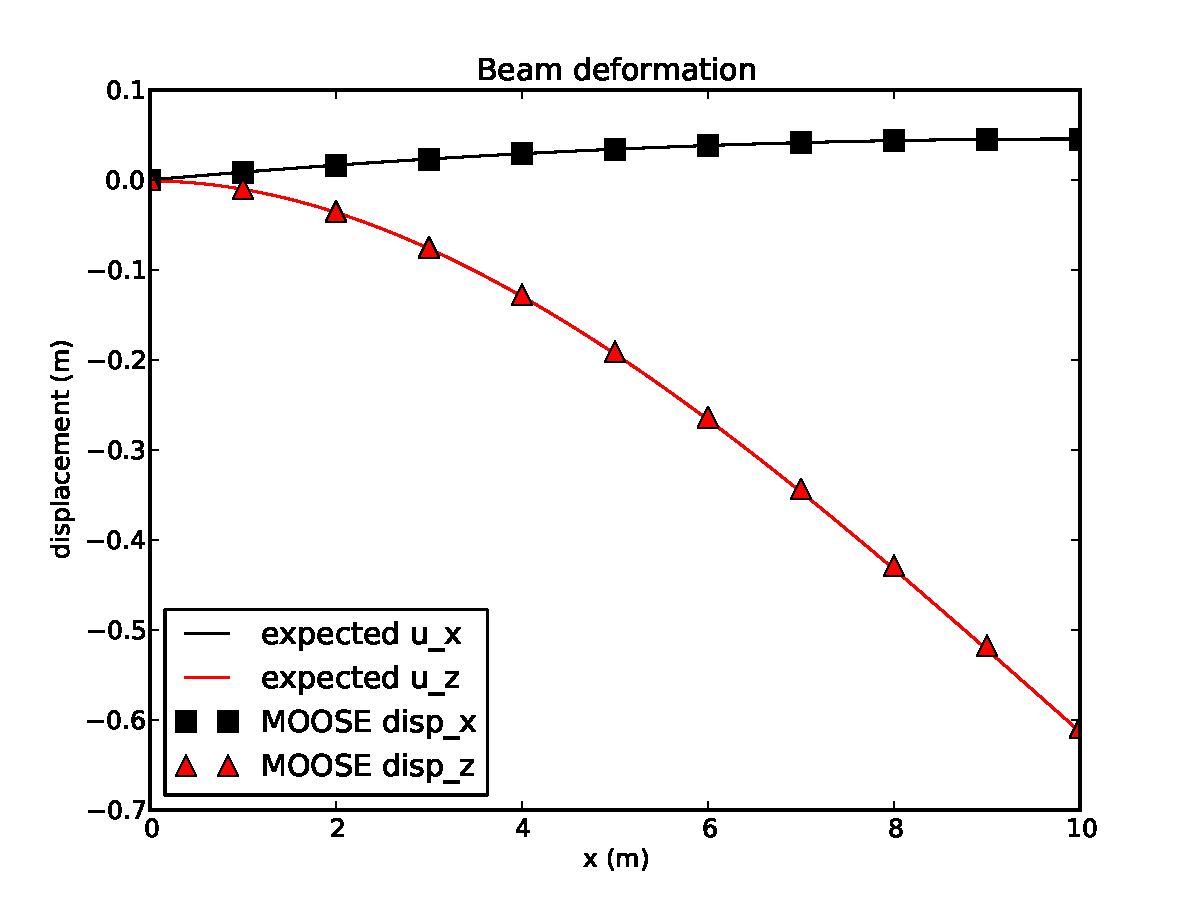
\includegraphics[width=8cm]{cosserat_beam_disp.pdf}
\caption{Displacements of the bar at $z=0.5$.  Here $L=10$, $c=0.5$,
  $E=1.2$, $\nu=0.3$ and $\tau=0.0002$.}
\label{cosserat_eam_disp.fig}
\end{center}
\end{figure}


\chapter{Beam bending 2}

A pure bend is applied to a the beam shown in
Figure~\ref{beam_cant.fig}.  In this section, the beam will be
modelled using a layered Cosserat material, with small Cosserat joint
shear stiffness (so that layers can slip over one another) and with
infinite normal stiffness.  Some of the material in this section can also be
found in Appendix B of Forest.\footnote{S Forest "Mechanics of
  Cosserat media An introduction".  Available from
  http://citeseerx.ist.psu.edu/viewdoc/download?doi=10.1.1.154.4476\&rep=rep1\&type=pdf}

Suppose that the beam is bent with the following deformations
\begin{eqnarray}
u_{x} & = & Axz \ , \\
u_{y} & = & Dzy \ , \\
u_{z} & = & -\mbox{$\frac{1}{2}$}Ax^{2} + \mbox{$\frac{1}{2}$}D(z^{2}
- y^{2})
\end{eqnarray}
To first order, in the $x$--$z$ plane, this is pure bending through an
arc of a circle:
\begin{equation}
(x, z) \rightarrow \left( (z+R)\frac{x}{\sqrt{x^{2}+R^{2}}},\,
(z+R)\frac{R}{\sqrt{x^{2}+R^{2}}} \right) \approx \left(x + xz/R,\,
 z -\mbox{$\frac{1}{2}$}x^{2}/R \right) \ ,
\end{equation}
with $A=1/R$.  The arbitrary constant $D$ and the deformation in the
$y$ direction are introduced so that plane
stress conditions ($\sigma_{yy}=0$) can be used.

The Cosserat layers are assumed to rotate along with the deformation,
that is
\begin{equation}
\theta_{c}^{i} = \mbox{$\frac{1}{2}$}\epsilon_{ijk}\partial_{j}u_{k}
\ ,
\end{equation}
meaning that
\begin{eqnarray}
\theta_{c}^{x} & = & -Dy \ , \\
\theta_{c}^{y} & = & Ax \ , \\
\theta_{c}^{z} & = & 0 \ .
\end{eqnarray}

The resulting nonzero strain and curvature components are
\begin{eqnarray}
\gamma_{xx} & = & Ax \ , \\
\gamma_{yy} & = & Dz \ , \\
\gamma_{zz} & = & Dz \ , \\
\kappa_{xy} & = & -D \ , \\
\kappa_{yx} & = & A
\end{eqnarray}
Finally, choosing
\begin{equation}
D = -\nu A
\end{equation}
(with $\nu$ being the Posson's ratio) gives, for layered Cosserat:
\begin{eqnarray}
\sigma_{xx} & = & AEz
\label{nonuniform.bend.stress} \ , \\
m_{yx} & = & \mbox{$\frac{1}{12}$}AEh^{2} \frac{G}{hk_{s} + G} \ .
\label{coss.mom.gen.eqn}
\end{eqnarray}
The other stress and moment-stress components are zero.  Here $G =
\frac{1}{2}E/(1+\nu)$ is the shear modulus, $h$ is the Cosserat layer
thickness and $k_{s}$ is the Cosserat joint shear stiffness.

Equation~(\ref{coss.mom.gen.eqn}) illustrates a key feature in Cosserat
mechanics.  The nonuniform stress of
Equation~(\ref{nonuniform.bend.stress}) is the standard (non-Cosserat)
way of producing pure circular bending in a bar.  Imagine that it is
applied to a single Cosserat layer of thickness $h$, as illustrated in
Figure~\ref{nonuniform_stress.fig}.  This generates a moment in the layer:
\begin{equation}
m_{yx} =
\frac{1}{hW}\int_{-W/2}^{W/2}\mathrm{d}y\int_{-h/2}^{h/2}\mathrm{d}z\,
AEz = \mbox{$\frac{1}{12}$}AEh^{2} \ ,
\label{eqn.mom.gen.zero}
\end{equation}
(for a depth $W$ in the $y$ direction).  The same result holds for a
layer that is not centred at $z=0$: the nonuniform stress
$\sigma_{xx}$ is decomposed into a uniform stretch and a varying part
that induces the micromechanical moment-stress.
Equation~(\ref{eqn.mom.gen.zero}) is exactly
Equation~(\ref{coss.mom.gen.eqn}) in the limit of zero Cosserat joint
shear stiffness.  A nonzero shear stiffness reduces the
micromechanical moment-stress that is generated in the Cosserat
layers.  Hence this example has revealed the meaning of the
moment-stresses in layered Cosserat mechanics: they are the moments
experienced by the layers the orginate from bending of the Cosserat layers.

\begin{figure}[htb]
\begin{center}
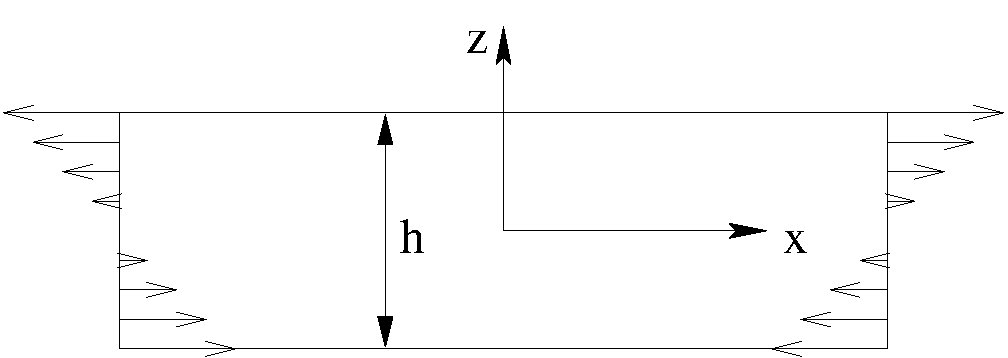
\includegraphics[width=8cm]{nonuniform_stress.pdf}
\caption{Stress $\sigma_{xx}=AEz$ is applied to a single Cosserat
  layer of thickness $h$}.
\label{nonuniform_stress.fig}
\end{center}
\end{figure}

The test suite contains two tests based on the above theory.  The
tests use $L=10$, $c=0.5$, $E=1.2$, $\nu=0.3$, $A=0.0111$ and $h=2$.
\begin{enumerate}
\item The deformations and Cosserat rotations are applied, and the
  stresses are measured to ensure that they satisfy
  Equations~(\ref{nonuniform.bend.stress})
  and~(\ref{coss.mom.gen.eqn}).  This test uses $k_{s}=\infty$.  This
  means $m_{yx}=0.00444$, and MOOSE produces this exactly.  MOOSE also
  produces the result for $\sigma_{xx}$, but the accuracy obviously
  depends on the resolution in the $z$ direction.

\item The $x=0$ end is held clamped, while $\sigma_{xx}$ and $m_{yz}$
  are applied to the right-hand end ($x=L$).  This test uses
  $k_{s}=0.1$.  There is no gaurantee that the expected deformations
  are indeed a minimum-energy configuration for the discretised
  situation, since small numerical discrepancies may cause MOOSE to
  fall into a different configuration.  This occurs if the number of
  elements in the $y$ direction is greater than 1: extra 3D effects appear
  --- twisting and wavy behaviour --- as moments are transferred
  between the Cosserat tensor, $m$, and the antisymmetric part of
  $\sigma$.  However, for one element in the $y$ direction, good
  agreement is obtained, as shown in Figure~\ref{beam2.fig}
\begin{figure}[htb]
\begin{center}
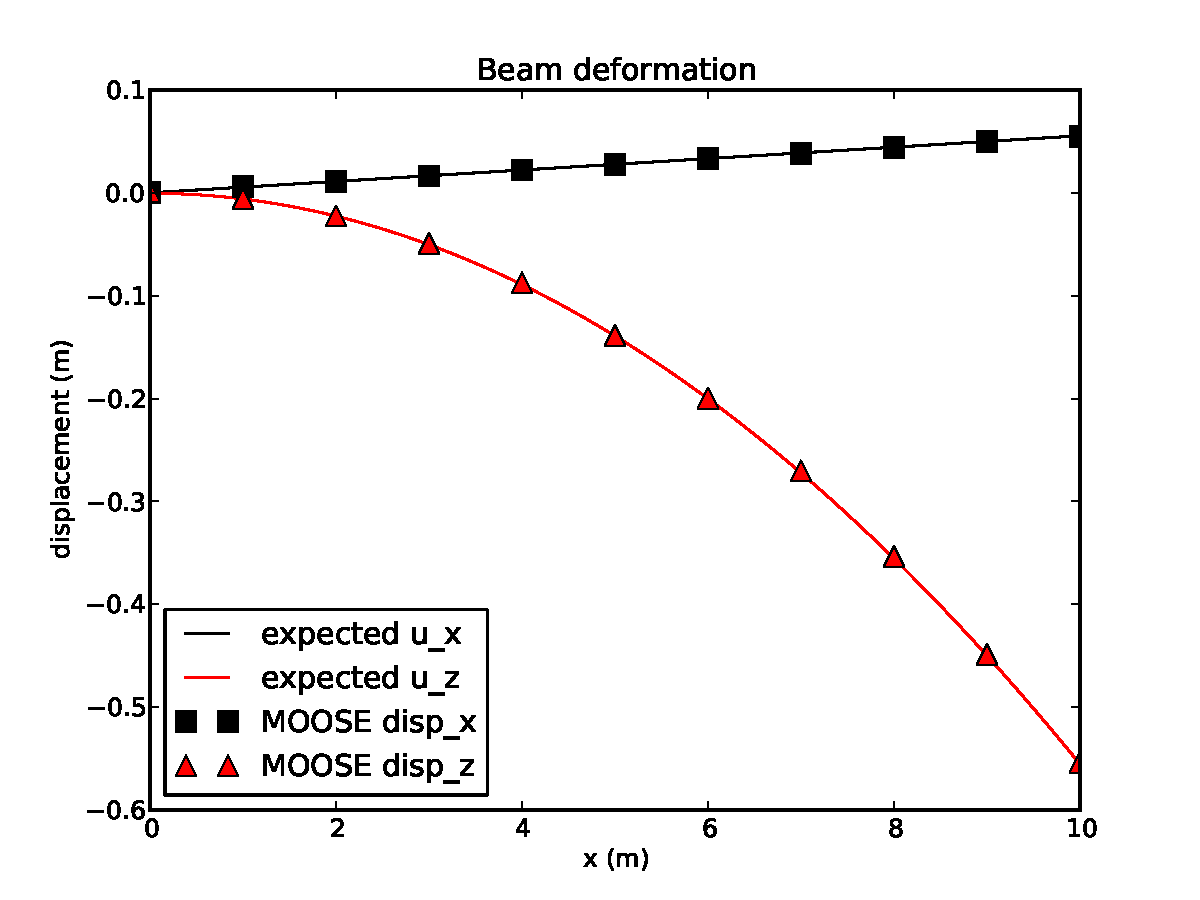
\includegraphics[width=8cm]{cosserat_beam_disp_2.pdf}
\caption{Deformations of the beam subjected to nonuniform
  $\sigma_{xx}$ and micromechanical moment-stress.}
\label{beam2.fig}
\end{center}
\end{figure}

\end{enumerate}

\end{document}

